\begin{figure}[ht]
\centering
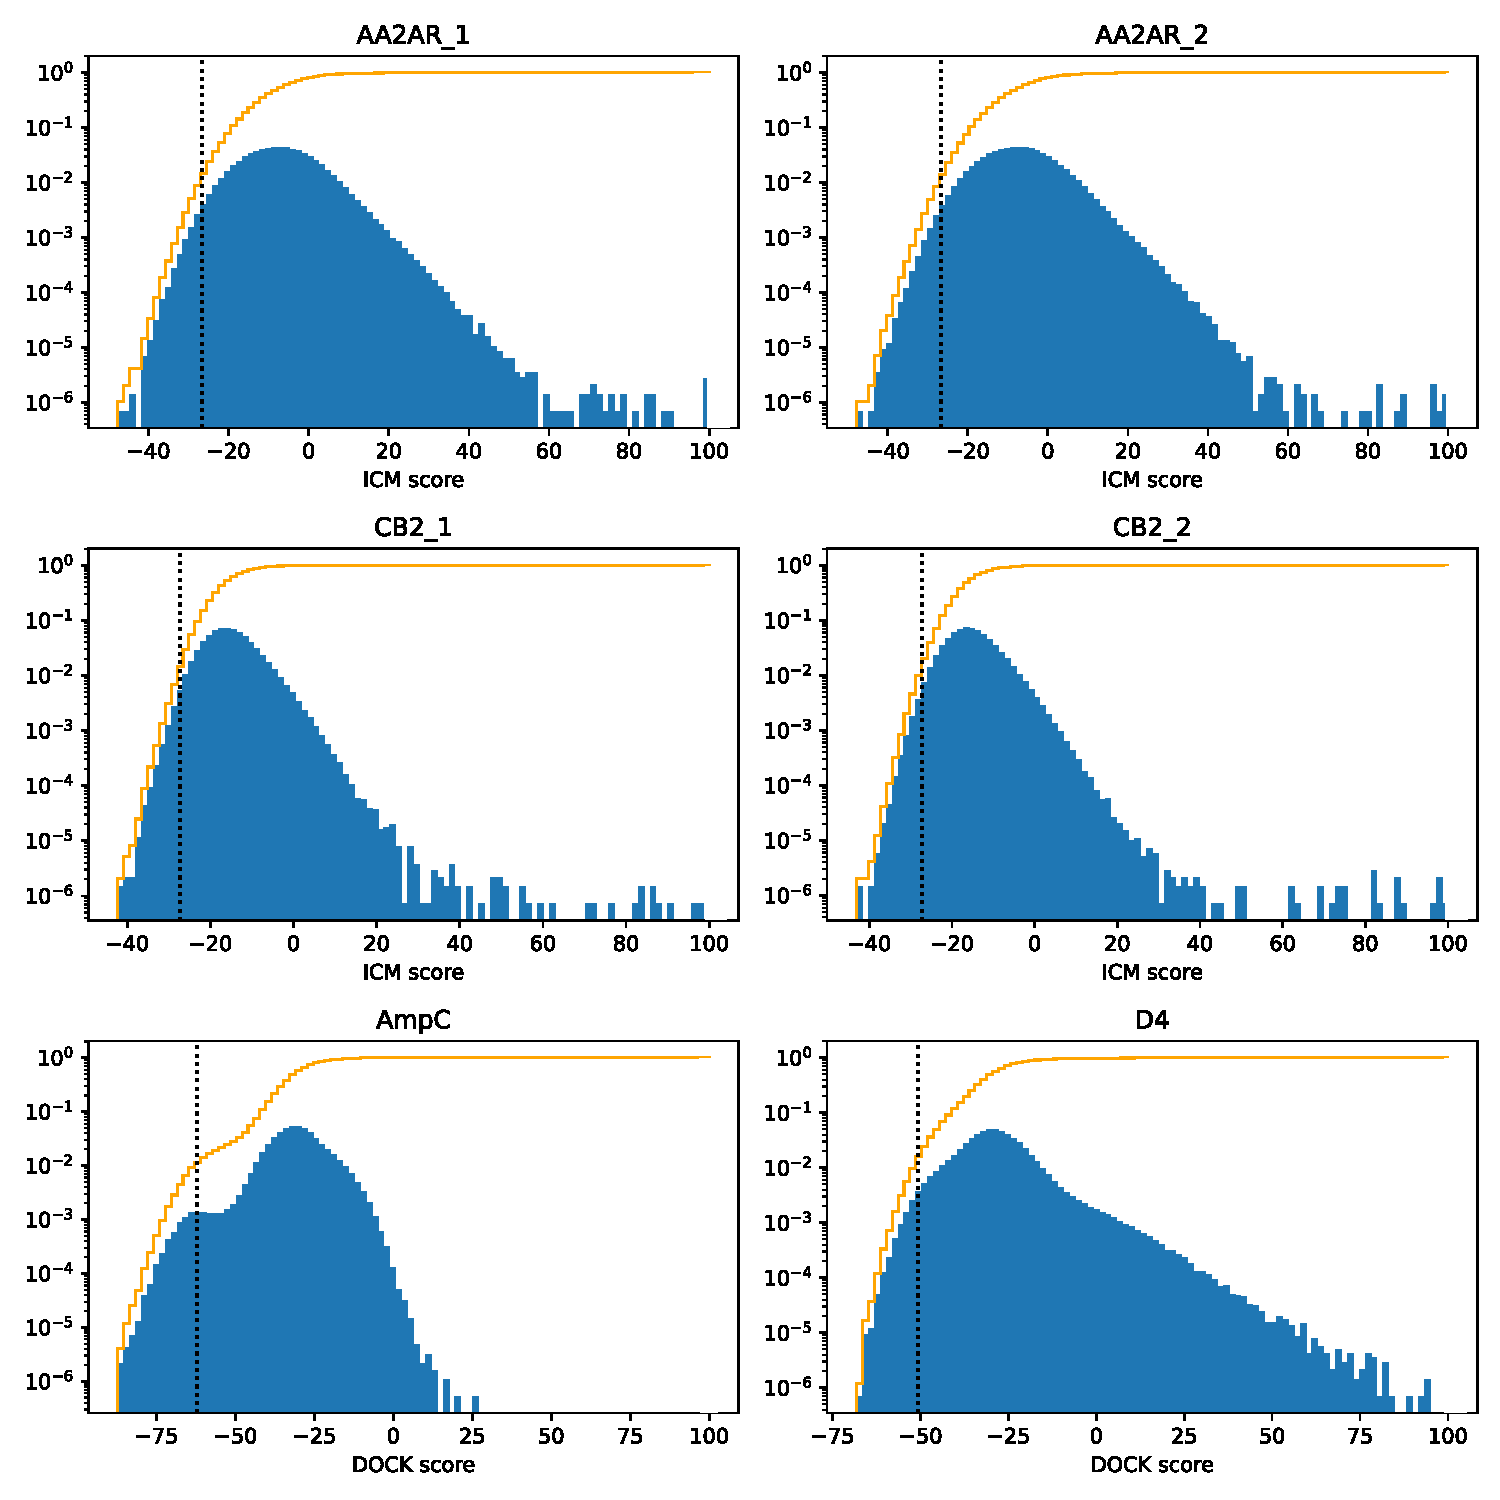
\includegraphics[width=1.0\textwidth]{figures/figure_1_scores_distribution_v3.pdf}
\caption{Distributions of scores for datasets used in the study. Histogram (blue) shows log-scale score distribution, while plot (orange) shows cumulative distribution of scores. Vertical line (black) shows cutoff for top-1\% of scores.}
\label{fig:fig_1_distribution}
\end{figure}


\begin{figure}[ht]
\centering
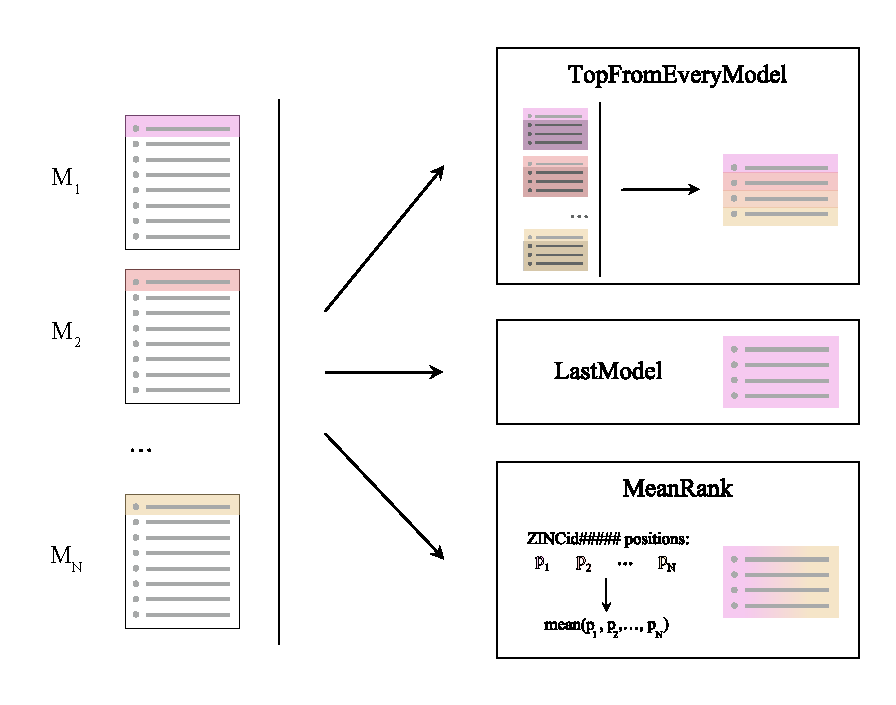
\includegraphics[width=1.0\textwidth]{figures/Figure_2_v4.pdf}
\caption{Overview of the active learning ranking schemes.}
\label{fig:fig_2_scheme}
\end{figure}


\begin{figure}[ht]
\centering
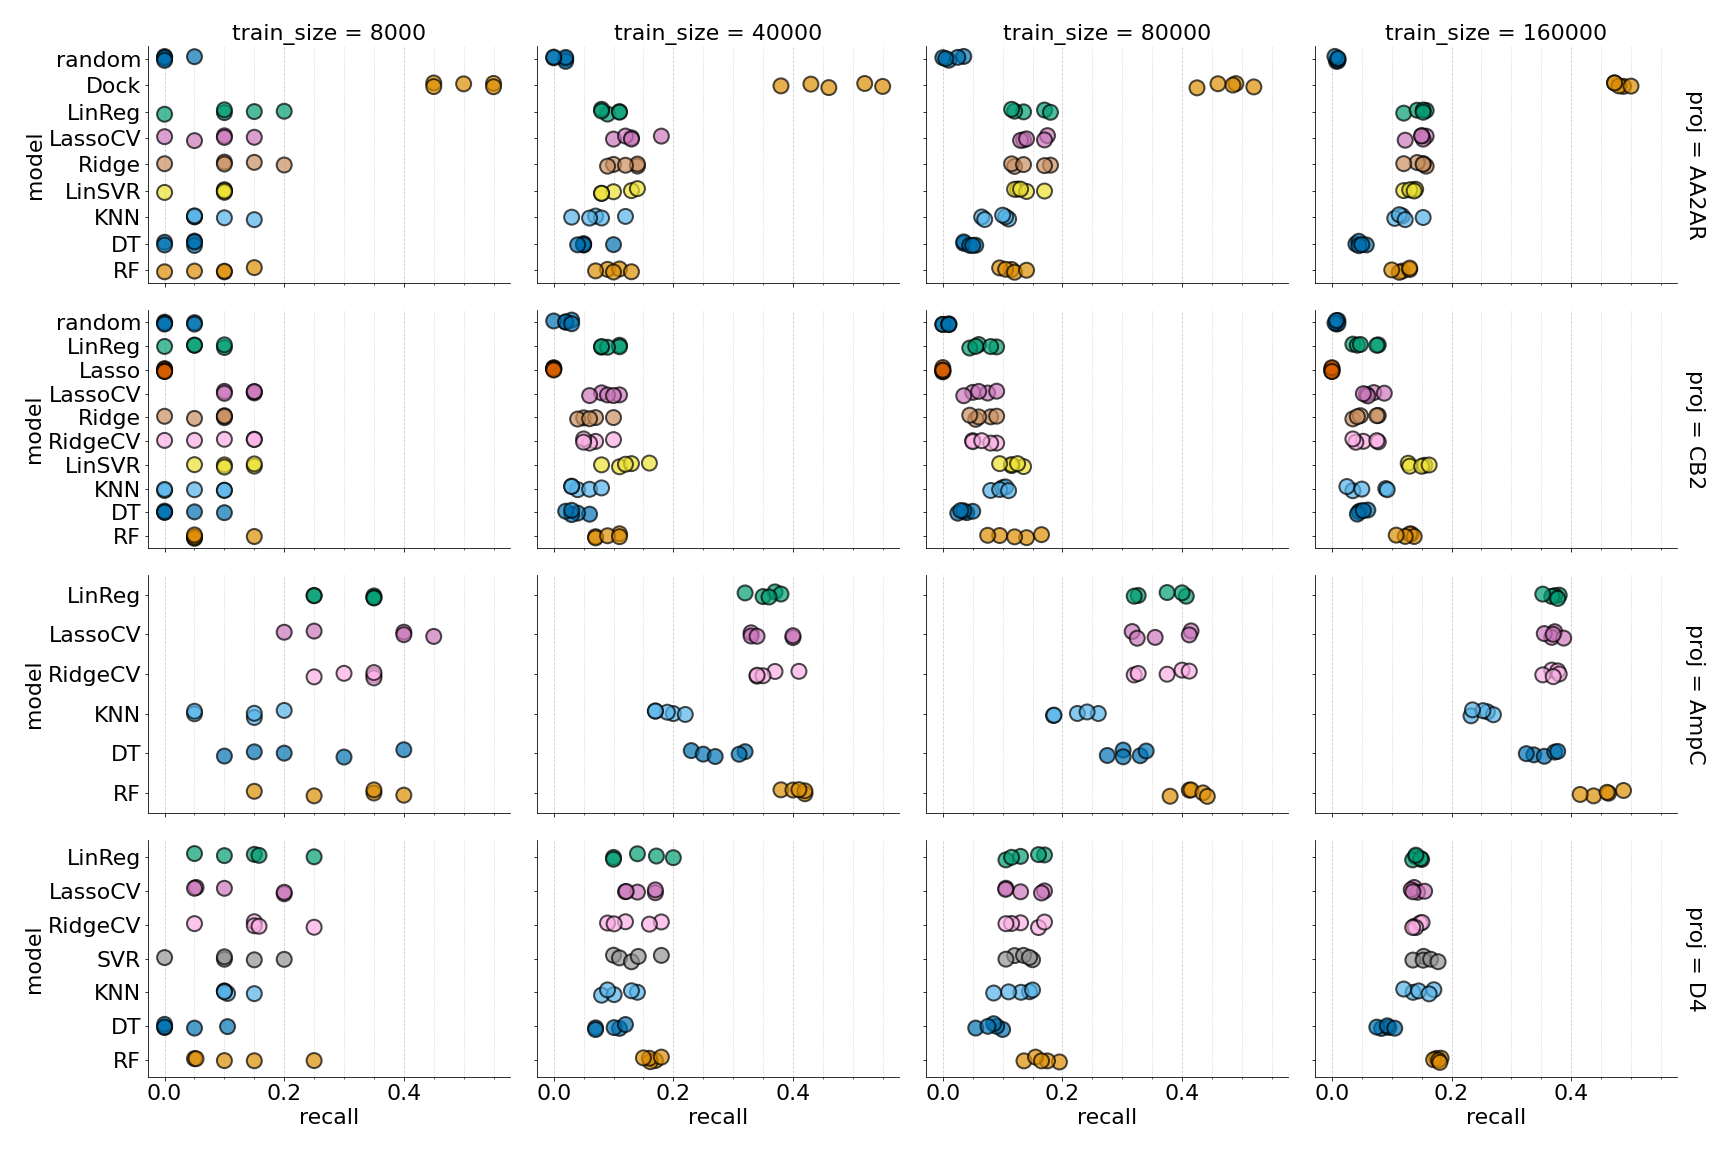
\includegraphics[width=1.0\textwidth]{figures/figure_3_single-shot-performance.png}
\caption{Model performance for multiple regression models and their baselines on 4 datasets present in the study. \texttt{recall\_score} shows the share of interception of top-1\% of the regressor's predictions with the actual top-1\%, sorted by docking score}
\label{fig:fig_3_singleshot}
\end{figure}


\begin{figure}[ht]
\centering
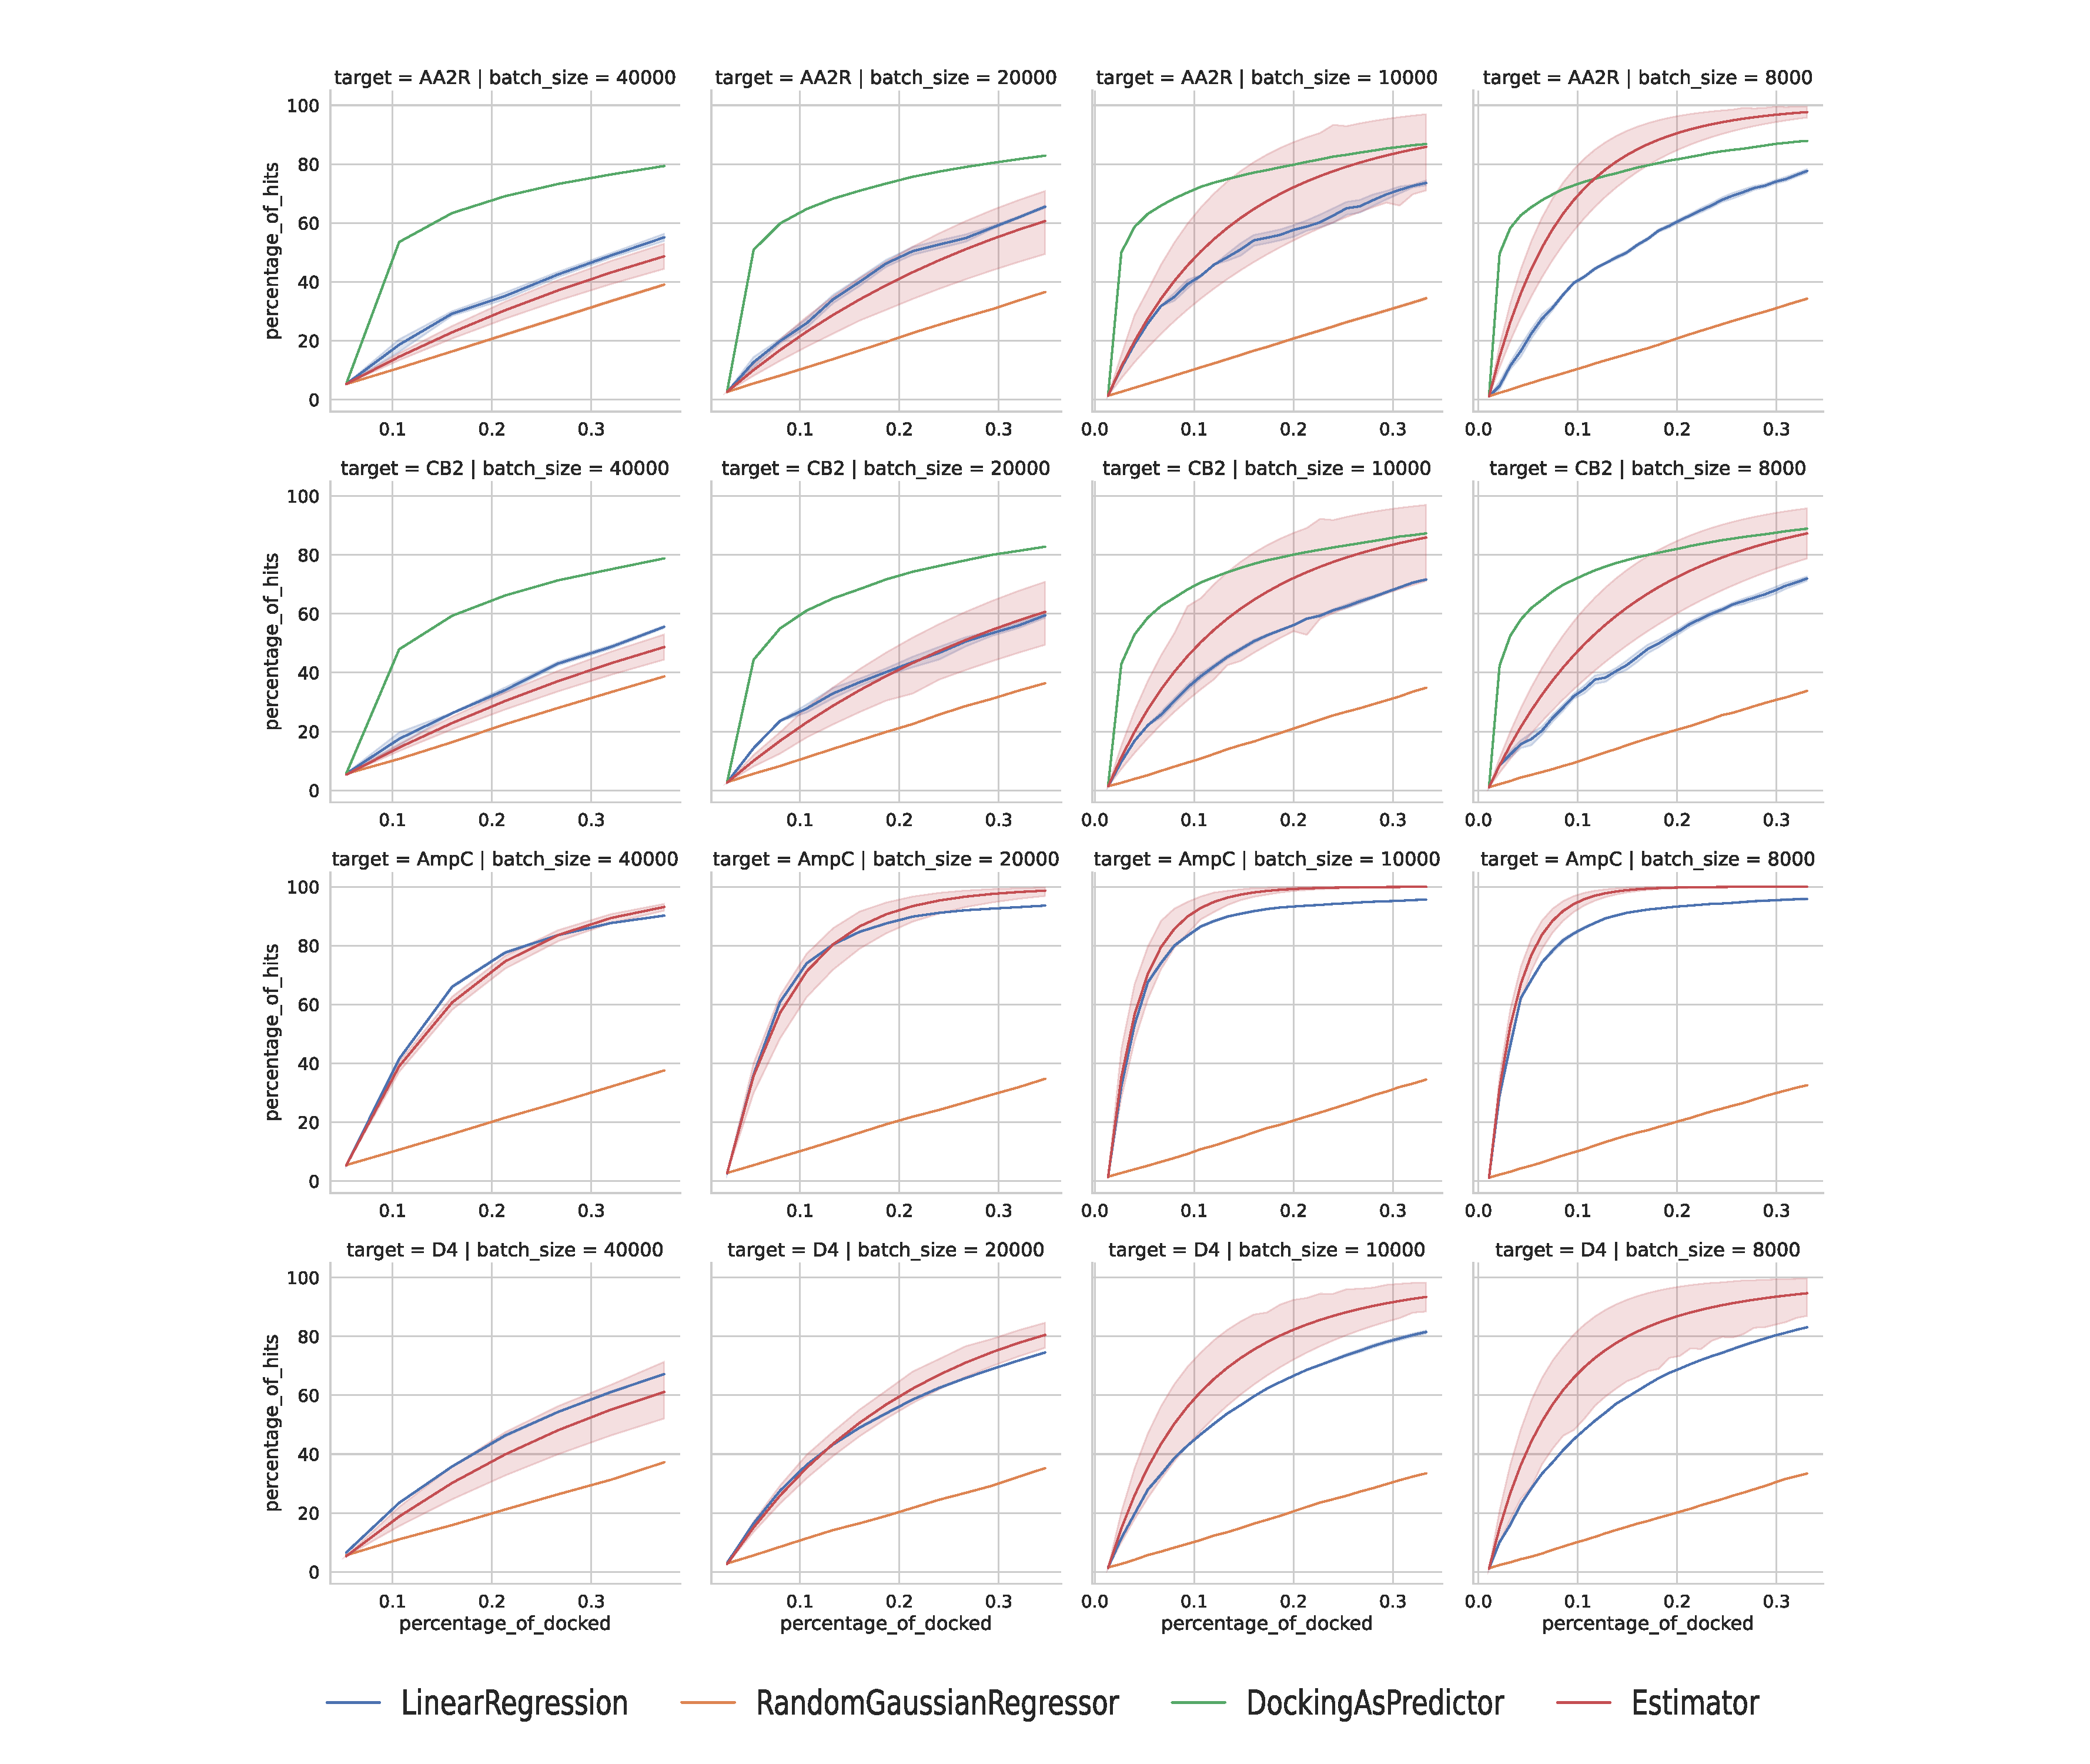
\includegraphics[width=1.0\textwidth]{figures/figure_4_iterations.pdf}
\caption{Model performance for multiple regression models and their baselines on 4 datasets present in the study. \texttt{recall\_score} shows the share of interception of top-1\% of the regressor's predictions with the actual top-1\%, sorted by docking score}
\label{fig:fig_4_extrapolation}
\end{figure}

\begin{table}[!ht]
    \centering
    \begin{adjustbox}{angle=90}
        \resizebox{1.2\textwidth}{!}
        {
            \begin{tabular}{|l|llllllllll|}
\hline
    \textbf{Compounds docked, \%} & \textbf{Batch size} & \textbf{Ensembling} & \textbf{Acquired hits, \%} & \textbf{} & \textbf{} & \textbf{} & \textbf{} & \textbf{} & \textbf{} & \textbf{} \\ \hline
    \textbf{} & ~ & ~ & AA2AR & ~ & CB2 & ~ & AmpC & ~ & D4 & ~ \\ 
    \textbf{} & ~ & ~ & “add” & “noadd” & “add” & “noadd” & “add” & “noadd” & “add” & “noadd” \\ 
    \textbf{10} & 40.000 & “LastModel” & 18 ± 4 & 19 ± 4 & 17 ± 5 & 17 ± 5 & 41.2 ± 0.2 & 41.6 ± 0.1 & 23.3 ± 0.5 & 23.5 ± 0.3 \\ 
    \textbf{} & ~ & “MeanRank” & 18 ± 4 & 18 ± 4 & 17 ± 5 & 17 ± 5 & 41.3 ± 0.3 & 41.2 ± 0.2 & 23.3 ± 0.5 & 23.4 ± 0.2 \\ 
    \textbf{} & ~ & “TopFromEveryModel” & 18 ± 3 & 18 ± 4 & 17 ± 5 & 17 ± 5 & 41.1 ± 0.2 & 41.2 ± 0.2 & 23 ± 1 & 23.3 ± 0.5 \\ 
    \textbf{} & ~ & Second docking & 53.8 ± 0.4 & 53.8 ± 0.2 & 47.57 ± 0.01 & 47.7 ± 0.3 & NA & NA & NA & NA \\ 
    \textbf{} & 20.000 & “LastModel” & 20 ± 8 & 26 ± 4 & 31.4 ± 0.3 & 28 ± 3 & 74.4 ± 0.4 & 74 ± 1 & 37.9 ± 0.1 & 36.35 ± 0.03 \\ 
    \textbf{} & ~ & “MeanRank” & 30 ± 7 & 28 ± 5 & 29.8 ± 0.5 & 30.5 ± 0.3 & 70 ± 1 & 72 ± 1 & 36.6 ± 0.2 & 37.8 ± 0.5 \\ 
    \textbf{} & ~ & “TopFromEveryModel” & 26 ± 8 & 25 ± 7 & 27 ± 2 & 28 ± 2 & 69.6 ± 0.4 & 70.6 ± 0.4 & 36.0 ± 0.3 & 35.6 ± 0.3 \\ 
    \textbf{} & ~ & Second docking & 64.8 ± 0.2 & 64.9 ± 0.2 & 61.1 ± 0.2 & 60.9 ± 0.3 & NA & NA & NA & NA \\ 
    \textbf{} & 10.000 & “LastModel” & 50 ± 2 & 42.1 ± 0.4 & 43 ± 3 & 39 ± 2 & 90.2 ± 0.1 & 87 ± 1 & 55.4 ± 0.3 & 46.7 ± 0.4 \\ 
    \textbf{} & ~ & “MeanRank” & 45 ± 4 & 48 ± 4 & 41 ± 1 & 44 ± 1 & 85 ± 1 & 88.6 ± 0.3 & 51.6 ± 0.4 & 54.0 ± 0.5 \\ 
    \textbf{} & ~ & “TopFromEveryModel” & 47 ± 2 & 43 ± 1 & 39 ± 6 & 36 ± 1 & 86 ± 1 & 85.3 ± 0.3 & 50.7 ± 0.3 & 47.0 ± 0.3 \\ 
    \textbf{} & ~ & Second docking & 72.25 ± 0.03 & 72.3 ± 0.1 & 70.4 ± 0.1 & 70.61 ± 0.03 & NA & NA & NA & NA \\ 
    \textbf{} & 8000 & “LastModel” & 45 ± 7 & 42 ± 1 & 40 ± 20 & 34 ± 3 & 92.4 ± 0.1 & 86 ± 1 & 61.8 ± 0.1 & 48.3 ± 0.3 \\ 
    \textbf{} & ~ & “MeanRank” & 40 ± 10 & 51 ± 3 & 39 ± 16 & 48 ± 3 & 88 ± 1 & 91.3 ± 0.4 & 56.7 ± 0.5 & 60 ± 1 \\ 
    \textbf{} & ~ & “TopFromEveryModel” & 40 ± 10 & 42 ± 3 & 40 ± 13 & 38 ± 1 & 89.2 ± 0.2 & 87.8 ± 0.3 & 56 ± 1 & 49.5 ± 0.4 \\ 
    \textbf{} & ~ & Second docking & 74.07 ± 0.02 & 74.1 ± 0.1 & 73.1 ± 0.1 & 73.2 ± 0.1 & NA & NA & NA & NA \\ 
    \textbf{30} & 40.000 & “LastModel” & 58 ± 2 & 55 ± 3 & 51 ± 4 & 56 ± 1 & 89.1 ± 0.3 & 90.2 ± 0.4 & 67.7 ± 0.3 & 67.2 ± 0.2 \\ 
    \textbf{} & ~ & “MeanRank” & 58 ± 4 & 56 ± 4 & 51 ± 5 & 53 ± 3 & 86.8 ± 0.5 & 87.8 ± 0.5 & 67 ± 1 & 68.0 ± 0.3 \\ 
    \textbf{} & ~ & “TopFromEveryModel” & 54 ± 6 & 57 ± 2 & 51 ± 7 & 53 ± 5 & 87.3 ± 0.2 & 88.4 ± 0.3 & 67± 1 & 67.1 ± 0.1 \\ 
    \textbf{} & ~ & Second docking & 79.7 ± 0.4 & 79.5 ± 0.2 & 78.5 ± 0.5 & 78.0 ± 1.0 & NA & NA & NA & NA \\ 
    \textbf{} & 20.000 & “LastModel” & 50 ± 15 & 66 ± 1 & 64 ± 2 & 60 ± 2 & 94.19 ± 0.02 & 93.6 ± 1e-14 & 76.1 ± 0.5 & 74.5 ± 0.4 \\ 
    \textbf{} & ~ & “MeanRank” & 62 ± 14 & 66 ± 3 & 63 ± 3 & 65 ± 3 & 92.3 ± 0.3 & 93.2 ± 0.4 & 74.8 ± 0.2 & 75.6 ± 0.4 \\ 
    \textbf{} & ~ & “TopFromEveryModel” & 63 ± 5 & 65 ± 3 & 63 ± 2 & 63 ± 2 & 93.1 ± 0.3 & 94.3 ± 0.2 & 74.6 ± 0.1 & 74.4 ± 0.4 \\ 
    \textbf{} & ~ & Second docking & 82.9 ± 0.2 & 82.7 ± 0.2 & 83.0 ± 0.1 & 82.9 ± 0.2 & NA & NA & NA & NA \\ 
    \textbf{} & 10.000 & “LastModel” & 79 ± 2 & 74 ± 2 & 73 ± 2 & 71.6 ± 0.4 & 97.0 ± 0.1 & 95.6 ± 0.1 & 85.6 ± 0.3 & 81 ± 1 \\ 
    \textbf{} & ~ & “MeanRank” & 70 ± 10 & 82 ± 1 & 73 ± 4 & 76.8 ± 0.2 & 96.2 ± 0.4 & 96.2 ± 0.2 & 84.3 ± 0.1 & 84.8 ± 0.2 \\ 
    \textbf{} & ~ & “TopFromEveryModel” & 78 ± 7 & 78 ± 1 & 68 ± 10 & 72 ± 1 & 96.8 ± 0.1 & 97.0 ± 0.1 & 84.1 ± 0.1 & 81.8 ± 0.2 \\ 
    \textbf{} & ~ & Second docking & 86.68 ± 0.01 & 86.80 ± 0.02 & 87.3 ± 0.1 & 87.5 ± 0.2 & NA & NA & NA & NA \\ 
    \textbf{} & 8000 & “LastModel” & 76 ± 10 & 78 ± 2 & 70 ± 20 & 72 ± 2 & 97.5 ± 0.1 & 96 ± 1 & 88.1 ± 0.4 & 83.1 ± 0.3 \\ 
    \textbf{} & ~ & “MeanRank” & 75 ± 6 & 85 ± 1 & 70 ± 20 & 80.3 ± 0.4 & 96.9 ± 0.1 & 96.8 ± 0.1 & 86.7 ± 0.1 & 87.6 ± 0.3 \\ 
    \textbf{} & ~ & “TopFromEveryModel” & 77 ± 5 & 80 ± 2 & 69 ± 15 & 75 ± 1 & 97.3 ± 0.1 & 97.5 ± 0.1 & 86.9 ± 0.2 & 84.0 ± 0.1 \\ 
    \textbf{} & ~ & Second docking & 88.1 ± 0.1 & 88.0 ± 0.1 & 88.8 ± 0.3 & 88.89 ± 0.01 & NA & NA & NA & NA \\ \hline
\end{tabular}

        }
    \end{adjustbox}
\end{table}

\begin{figure}[ht]
\centering
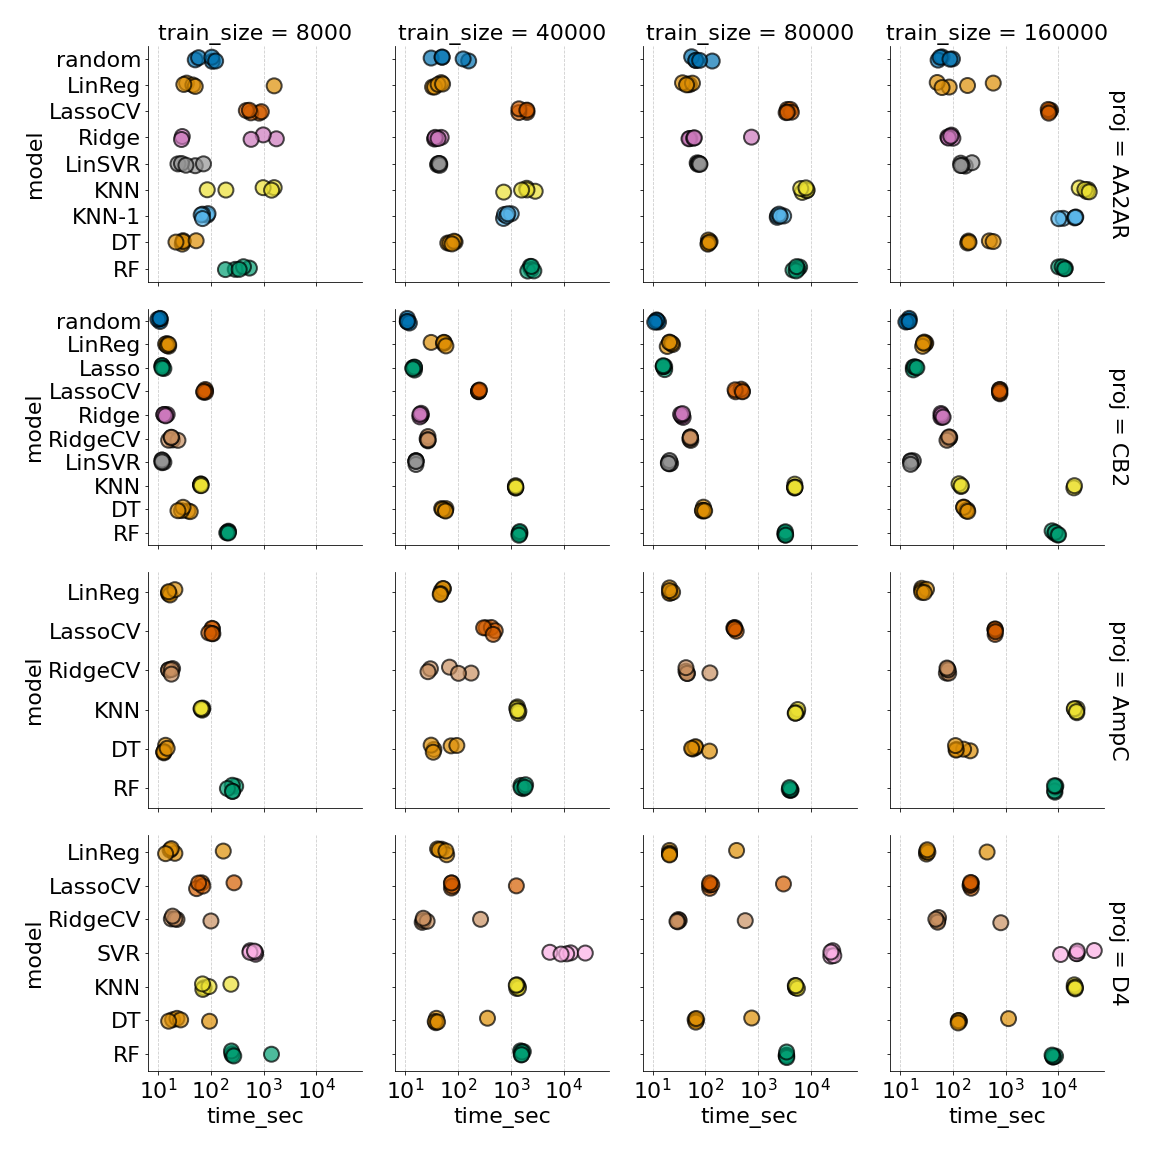
\includegraphics[width=1.0\textwidth]{figures/Supp_Figure_1_execution_time.png}
\caption{Execution time (log scale) of the train-predict loop of the algorithms evaluated in single-shot regime.}
\label{fig:supp_fig_1_execution_time}
\end{figure}
